\section{Resultados: RQ01 a RQ04}
\label{sec:resultados-a}

% Gerado por analises.sprint3_a; não edite à mão.
\newcommand{\labAFreqMediana}{0,326}
\newcommand{\labAFreqQUm}{0,153}
\newcommand{\labAFreqQTres}{0,825}
\newcommand{\labAFreqMaximo}{14,364}
\newcommand{\labAFreqN}{300}
\newcommand{\labAFreqPreMediana}{0,345}
\newcommand{\labAFreqPreQUm}{0,173}
\newcommand{\labAFreqPreQTres}{0,863}
\newcommand{\labAFreqPreMaximo}{71,707}
\newcommand{\labAFreqPreN}{300}
\newcommand{\labAFreqTagsMediana}{0,403}
\newcommand{\labAFreqTagsQUm}{0,192}
\newcommand{\labAFreqTagsQTres}{1,016}
\newcommand{\labAFreqTagsMaximo}{76,329}
\newcommand{\labAFreqTagsN}{300}
\newcommand{\labAFreqDiarios}{3}
\newcommand{\labAFreqSemanais}{56}
\newcommand{\labAFreqSemanaisPct}{18,7}
\newcommand{\labAFreqPreXMaior}{87}
\newcommand{\labAFreqPreIguais}{213}
\newcommand{\labAFreqPreXMenor}{0}
\newcommand{\labAFreqPreDifMediana}{0,000}
\newcommand{\labAFreqPreRazao}{1,00}
\newcommand{\labAFreqPreR}{--}
\newcommand{\labAFreqPrePHolm}{--}
\newcommand{\labAFreqTagsXMaior}{162}
\newcommand{\labAFreqTagsIguais}{135}
\newcommand{\labAFreqTagsXMenor}{3}
\newcommand{\labAFreqTagsDifMediana}{0,019}
\newcommand{\labAFreqTagsRazao}{1,02}
\newcommand{\labAFreqTagsR}{--}
\newcommand{\labAFreqTagsPHolm}{--}
\newcommand{\labALeadAMediana}{196,7}
\newcommand{\labALeadAQUm}{47,26}
\newcommand{\labALeadAQTres}{715,6}
\newcommand{\labALeadAMaximo}{40.129,8}
\newcommand{\labALeadAN}{300}
\newcommand{\labALeadBMediana}{178,3}
\newcommand{\labALeadBQUm}{43,10}
\newcommand{\labALeadBQTres}{475,4}
\newcommand{\labALeadBMaximo}{34.894,6}
\newcommand{\labALeadBN}{300}
\newcommand{\labALeadXMaior}{191}
\newcommand{\labALeadIguais}{2}
\newcommand{\labALeadXMenor}{107}
\newcommand{\labALeadDifMediana}{24,84}
\newcommand{\labALeadRazao}{1,49}
\newcommand{\labALeadR}{0,325}
\newcommand{\labALeadPHolm}{$1,12\times 10^{-6}$}
\newcommand{\labACfrAMediana}{0,055}
\newcommand{\labACfrAQUm}{0,024}
\newcommand{\labACfrAQTres}{0,129}
\newcommand{\labACfrAMaximo}{0,953}
\newcommand{\labACfrAN}{300}
\newcommand{\labACfrBMediana}{0,175}
\newcommand{\labACfrBQUm}{0,000}
\newcommand{\labACfrBQTres}{0,429}
\newcommand{\labACfrBMaximo}{1,000}
\newcommand{\labACfrBN}{289}
\newcommand{\labACfrBAusentes}{11}
\newcommand{\labACfrBZeros}{74}
\newcommand{\labACfrBZerosPct}{25,6}
\newcommand{\labACfrAZeros}{16}
\newcommand{\labACfrXMaior}{101}
\newcommand{\labACfrIguais}{2}
\newcommand{\labACfrXMenor}{186}
\newcommand{\labACfrDifMediana}{$-$0,109}
\newcommand{\labACfrRazao}{--}
\newcommand{\labACfrR}{$-$0,554}
\newcommand{\labACfrPHolm}{$8,13\times 10^{-16}$}
\newcommand{\labARecMediana}{3,20}
\newcommand{\labARecQUm}{0,60}
\newcommand{\labARecQTres}{18,37}
\newcommand{\labARecMaximo}{2.627,0}
\newcommand{\labARecN}{278}
\newcommand{\labARecAusentes}{22}
\newcommand{\labAEpMediana}{3,57}
\newcommand{\labAEpQUm}{0,88}
\newcommand{\labAEpQTres}{20,28}
\newcommand{\labAEpMaximo}{6.019,4}
\newcommand{\labAEpN}{7.771}
\newcommand{\labAEpTotal}{7.861}
\newcommand{\labAEpCensurados}{90}
\newcommand{\labAEpCensuradosPct}{1,1}
\newcommand{\labAEpPNoventa}{73,37}
\newcommand{\labAEpDiaPct}{21,3}
\newcommand{\labAEpSemanaPct}{4,2}
\newcommand{\labAEpPiorCaso}{3,66}
\newcommand{\labARecPiorCaso}{3,33}
\newcommand{\labARepoCensura}{61}
\newcommand{\labARepoCensuraPct}{21,9}
\newcommand{\labARepoSemEpisodios}{22}


Cada projeto contribui com uma observação por métrica; as distribuições são resumidas
por mediana e intervalo interquartil (IQR), sem médias. Ausências não são imputadas: o
CFR~(b) existe para \labACfrBN\ projetos e o tempo de recuperação para \labARecN.
A Tabela~\ref{tab:rq01-04} reúne todas as variantes, e a Figura~\ref{fig:rq01-04} mostra
as distribuições com os cortes da classificação DORA de referência.

\begin{table}[htbp]
\centering\footnotesize
\caption{RQ01 a RQ04: mediana e quartis de cada variante. Uma observação por projeto,
exceto na última linha, que reúne os episódios concluídos.}
\label{tab:rq01-04}
% Gerado por analises.sprint3_a; não edite à mão.
\begin{tabular}{lllrrrr}
\hline
RQ & Métrica & Unidade & $n$ & Mediana & Q1--Q3 & IQR \\
\hline
RQ01 & Frequência: releases & por semana & 300 & 0,326 & 0,153--0,825 & 0,671 \\
RQ01 & Frequência: com pré-releases & por semana & 300 & 0,345 & 0,173--0,863 & 0,690 \\
RQ01 & Frequência: tags & por semana & 300 & 0,403 & 0,192--1,016 & 0,825 \\
\hline
RQ02 & Lead time (a): por release & horas & 300 & 196,7 & 47,26--715,6 & 668,3 \\
RQ02 & Lead time (b): por commit & horas & 300 & 178,3 & 43,10--475,4 & 432,3 \\
\hline
RQ03 & CFR (a): runs de CI & proporção & 300 & 0,055 & 0,024--0,129 & 0,105 \\
RQ03 & CFR (b): releases & proporção & 289 & 0,175 & 0,000--0,429 & 0,429 \\
\hline
RQ04 & Recuperação: mediana por projeto & horas & 278 & 3,20 & 0,60--18,37 & 17,77 \\
RQ04 & Recuperação: episódios concluídos & horas & 7.771 & 3,57 & 0,88--20,28 & 19,40 \\
\hline
\end{tabular}

\end{table}

\begin{figure}[htbp]
\centering
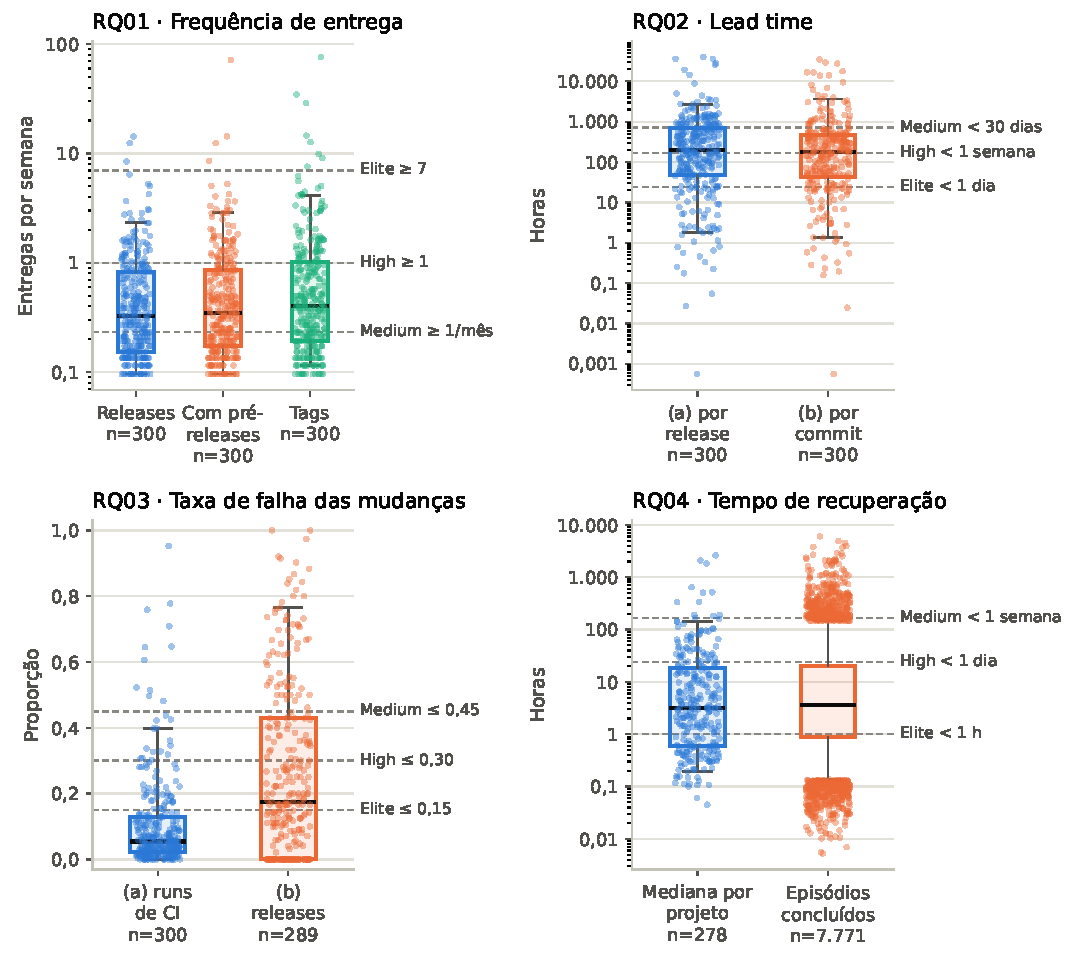
\includegraphics[width=\textwidth]{../../results/s03_a/rq01_04_distribuicoes.pdf}
\caption{Distribuições das RQ01 a RQ04. Caixas: Q1, mediana e Q3; bigodes nos percentis
5 e 95; pontos são projetos (nos episódios, apenas valores fora de P5--P95). Linhas
tracejadas marcam os cortes da classificação DORA. Escala logarítmica, exceto no CFR.}
\label{fig:rq01-04}
\end{figure}

\subsection{RQ01: frequência de entrega}

A mediana é de \labAFreqMediana\ release principal por semana (Q1--Q3:
\labAFreqQUm--\labAFreqQTres), cerca de uma release a cada três semanas. Somente
\labAFreqSemanais\ projetos (\labAFreqSemanaisPct\%) publicam ao menos uma por semana,
e apenas \labAFreqDiarios\ chegam a sete ou mais; o máximo é \labAFreqMaximo. Incluir
pré-releases altera a frequência de \labAFreqPreXMaior\ projetos, mas pouco a mediana
(\labAFreqPreMediana). Contar tags aumenta a frequência de \labAFreqTagsXMaior\ projetos
(mediana \labAFreqTagsMediana): parte das versões é marcada sem release publicada.
\textbf{H1 é sustentada}: a mediana fica abaixo de uma release por semana, com cauda
longa à direita.

\subsection{RQ02: lead time}

O lead time mediano é de \labALeadAMediana\ horas na variante~(a), cerca de oito dias,
e de \labALeadBMediana\ horas na~(b). A Tabela~\ref{tab:rq01-04-pares} compara as
variantes no mesmo projeto: (a) supera (b) em \labALeadXMaior\ de \labALeadAN\ projetos
(Wilcoxon pareado; $p$ ajustado por Holm de \labALeadPHolm; correlação rank-biserial
$r$ = \labALeadR), com razão mediana de \labALeadRazao. A diferença mediana, porém, é de
\labALeadDifMediana\ horas, e em \labALeadXMenor\ projetos a variante~(b) é a maior.

\begin{table}[htbp]
\centering\footnotesize
\caption{Variantes no mesmo projeto. $r$: correlação rank-biserial pareada; Wilcoxon e
Holm só nas comparações das hipóteses H2 e H3.}
\label{tab:rq01-04-pares}
% Gerado por analises.sprint3_a; não edite à mão.
\begin{tabular}{lrrrrrrr}
\hline
Diferença $x-y$ & $n$ & $x>y$ & $x=y$ & $x<y$ & Mediana & $r$ & $p$ Holm \\
\hline
Com pré-releases $-$ releases & 300 & 87 & 213 & 0 & 0,000 & -- & -- \\
Tags $-$ releases & 300 & 162 & 135 & 3 & 0,019 & -- & -- \\
Lead time (a) $-$ (b), horas & 300 & 191 & 2 & 107 & 24,84 & 0,325 & $1,12\times 10^{-6}$ \\
CFR (a) $-$ CFR (b) & 289 & 101 & 2 & 186 & $-$0,109 & $-$0,554 & $8,13\times 10^{-16}$ \\
\hline
\end{tabular}

\end{table}

A H2 supunha que a variante~(b) seria dominada por commits escritos perto da publicação.
Isso não ocorre porque (b) pondera cada release pelo número de commits, enquanto (a) dá
o mesmo peso a todas. Nas \labALeadReleases\ releases com commits válidos, quanto mais
commits, mais antigo é o primeiro deles: o Spearman entre as duas grandezas tem mediana de
\labALeadRhoMediano\ nos \labALeadProjetosRho\ projetos avaliáveis e é positivo em
\labALeadRhoPositivosPct\% deles. As releases longas, que acumulam muitas mudanças,
contribuem com a maior parte dos pares de~(b) e a aproximam de~(a). Em
\labALeadUmCommitPct\% das releases há um único commit, e as duas medidas coincidem.
\textbf{H2 é parcialmente sustentada}: (a) tende a ser maior, mas não muito maior.

\subsection{RQ03: taxa de falha das mudanças}

O CFR~(a) mediano é \labACfrAMediana\ (Q1--Q3: \labACfrAQUm--\labACfrAQTres): na maioria
dos projetos, poucos runs de CI do default branch falham. O CFR~(b) mediano é
\labACfrBMediana\ (\labACfrBQUm--\labACfrBQTres) e é mais disperso: \labACfrBZeros\ projetos
(\labACfrBZerosPct\%) não têm release seguida de corretiva, e um quarto dos projetos
passa de \labACfrBQTres. No mesmo projeto, (b) supera (a) em \labACfrXMenor\ de \labACfrBN\ casos
($p$ ajustado de \labACfrPHolm; $r$ = \labACfrR). \textbf{H3 não é sustentada; ocorre o
inverso.}

Os dois proxies observam falhas diferentes. Uma falha de CI no default branch interrompe
a integração, mas não chega ao usuário, e parte dos problemas já é barrada nas revisões
de pull request antes do merge. Uma release corretiva em até sete dias indica que uma
versão entregue precisou de conserto, o que está mais próximo da noção DORA de falha em
produção. Ainda assim, ela depende da heurística e de um denominador pequeno: com poucas
releases por projeto, cada corretiva move muito a taxa. Nenhum dos dois mede incidentes
em produção.

\subsection{RQ04: tempo de recuperação}

A mediana por projeto é de \labARecMediana\ horas (Q1--Q3: \labARecQUm--\labARecQTres),
e a dos \labAEpN\ episódios concluídos, de \labAEpMediana\ horas. A cauda é pesada: o
percentil 90 dos episódios é \labAEpPNoventa\ horas, \labAEpDiaPct\% duram um dia ou
mais, \labAEpSemanaPct\% uma semana ou mais, e o mais longo chega a \labAEpMaximo\ horas.
Apenas \labAEpCensurados\ dos \labAEpTotal\ episódios (\labAEpCensuradosPct\%) estão
censurados, distribuídos em \labARepoCensura\ projetos (\labARepoCensuraPct\% dos que
têm episódios). Mesmo supondo que cada episódio censurado dure mais que todos os
concluídos, a mediana dos episódios passaria a \labAEpPiorCaso\ horas, e a mediana por
projeto, a \labARecPiorCaso\ horas. Os \labARepoSemEpisodios\ projetos sem episódio
observável não têm tempo de recuperação, o que não equivale a recuperação instantânea.
\textbf{H4 é parcialmente sustentada}: a recuperação típica leva poucas horas e tem cauda
pesada, mas a censura é pequena e quase não afeta a mediana.

\subsection{Classificação de referência (C1)}

A combinação C1 usa releases principais, lead time~(a), CFR~(a) e tempo de recuperação,
com as faixas da tabela de referência; a categoria geral é a mediana das quatro notas
(Elite = 4 a Low = 1), arredondada para baixo. A Tabela~\ref{tab:c1} e a
Figura~\ref{fig:c1} apresentam a distribuição.

\begin{table}[htbp]
\centering\footnotesize
\caption{Classificação C1 por métrica e geral (porcentagem sobre 300 projetos). A última
linha é uma sensibilidade que aceita três métricas.}
\label{tab:c1}
% Gerado por analises.sprint3_a; não edite à mão.
\begin{tabular}{lrrrrr}
\hline
Dimensão & Elite & High & Medium & Low & Sem categoria \\
\hline
Frequência & 3 (1,0\%) & 53 (17,7\%) & 122 (40,7\%) & 122 (40,7\%) & 0 (0,0\%) \\
Lead time (a) & 57 (19,0\%) & 84 (28,0\%) & 85 (28,3\%) & 74 (24,7\%) & 0 (0,0\%) \\
CFR (a) & 235 (78,3\%) & 40 (13,3\%) & 14 (4,7\%) & 11 (3,7\%) & 0 (0,0\%) \\
Recuperação & 85 (28,3\%) & 133 (44,3\%) & 49 (16,3\%) & 11 (3,7\%) & 22 (7,3\%) \\
Geral & 17 (5,7\%) & 122 (40,7\%) & 110 (36,7\%) & 29 (9,7\%) & 22 (7,3\%) \\
\hline
Geral ($\geq$ 3 métricas) & 24 (8,0\%) & 128 (42,7\%) & 114 (38,0\%) & 34 (11,3\%) & 0 (0,0\%) \\
\hline
\end{tabular}

\end{table}

\begin{figure}[htbp]
\centering
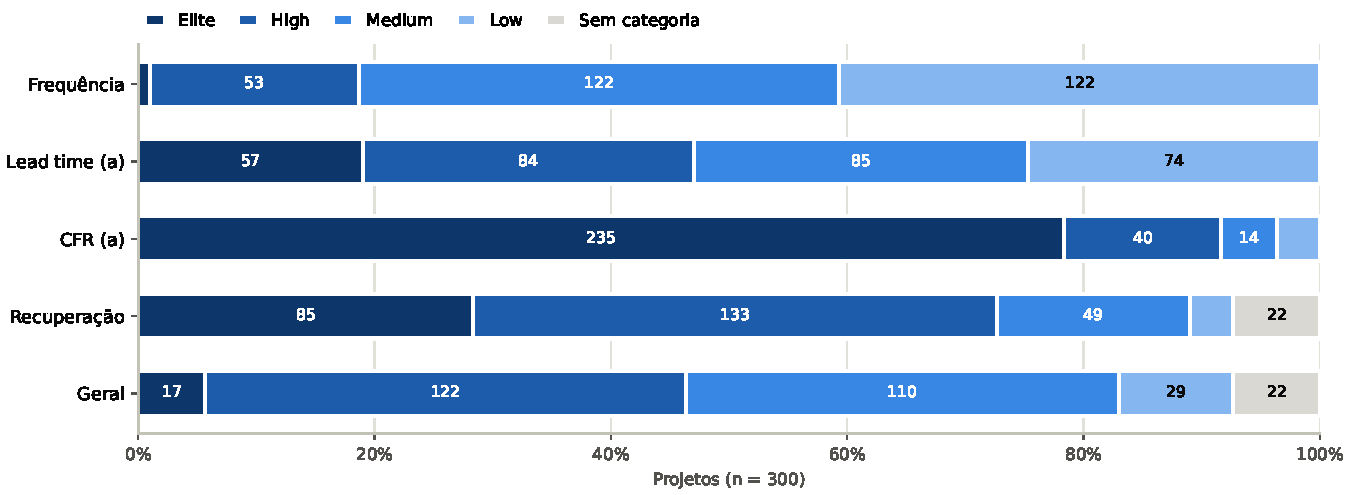
\includegraphics[width=\textwidth]{../../results/s03_a/c1_distribuicao.pdf}
\caption{Classificação C1. Segmentos sem rótulo têm menos de 14 projetos; os valores
estão na Tabela~\ref{tab:c1}.}
\label{fig:c1}
\end{figure}

A frequência é a dimensão mais fraca: \labACOneFreqElite\ projetos são Elite, e
\labACOneFreqMediumPct\% e \labACOneFreqLowPct\% ficam em Medium e Low, respectivamente.
O CFR~(a) é a mais favorável, com \labACOneCfrElitePct\% em Elite. O lead time~(a)
se distribui pelas quatro categorias, e a recuperação se concentra em High
(\labACOneRecHighPct\%). Na classificação geral predominam High (\labACOneGeralHigh) e
Medium (\labACOneGeralMedium); \labACOneGeralElite\ projetos são Elite e
\labACOneGeralLow\ são Low.

Os \labACOneGeralSem\ projetos sem episódio de recuperação ficam sem categoria geral,
pois a definição principal exige as quatro métricas. Classificados com as três
disponíveis, eles se distribuiriam entre Elite (\labACOneSemGeralElite), High
(\labACOneSemGeralHigh), Medium (\labACOneSemGeralMedium) e Low (\labACOneSemGeralLow),
sem concentrar a exclusão em uma categoria. Em \labACOneFracionarias\ dos
\labACOneClassificados\ projetos classificados (\labACOneFracionariasPct\%), as duas
notas centrais diferem e o arredondamento decide a categoria: são casos próximos de um
limite, sensíveis à definição operacional avaliada na RQ07.
